%
% Memory based reasoning - Project
% Report
%
% created: 27. April 2012
%
\documentclass[11pt]{article}
\usepackage[T1]{fontenc}
\usepackage{graphicx}

%\usepackage{hyperref}
%\hypersetup{
%    colorlinks,
%    citecolor=black,
%    filecolor=black,
%    linkcolor=black,
%    urlcolor=black
%}

\title{
	\emph{A Report for}\\
	\huge{\textbf{Footprint-Based Retrieval} }\\
	-Project-\\
	Memory-Based Reasoning in AI\\[2em]	
}
\author{
	Philipp Fonteyn (MS11F010)\\
	Saurabh Baghel (CS12D003)\\[2em]
	%\emph{Master of Technology}\\
	\emph{Computer Science \& Engineering, IIT Madras}
}
\date{3rd of May 2012}

\makeatletter
\g@addto@macro\@verbatim\small
\makeatother 


%
% Document
%
\begin{document}
\maketitle
\newpage
%\tableofcontents
%\newpage

%
%
%
\section{Introduction}
Systems using Case-Based Reasoning (CBR) compare already existing solved problems in a normally large case-base in order to find similar cases and therefore suitable solutions for the problem at hand. If one wants to evaluate the quality of such a system he would have to look for the efficiency and the quality of the retrieval process. We have a trade off between retrieval time and the usability or adaptability of the found solution for the problem at hand. Because of this the research in this area is still an ongoing and interesting one.
%
%
%
\section{The Footprint-Based Approach}
To search and retrieve the case-base there are several approaches to structure and traverse the data. In this project we will concentrate on the so called "Footprint-based" (FPB) approach introduced by Smyth and McKenna \cite{FPBR}. The main idea of this approach is to exploit the growing clusters in a case base such that so called "correspondence groups" evolve. A footprint of the case-base is then a subset of the case-base that covers all the existing correspondence groups. In the end iteratively the footprint will be generated. The retrieval process itself then has two major parts. First it identifies the local group with highest correspondence and then searches for the best suited target. 

\subsection{Used Subsets}

\subsection{The algorithm}
describe the FBR algorithm

%
%
% THAT WAS OUR OUTLOOK:
%\section{Outlook on the project}
%
%\textbf{Description of domain} - In the following report of this project we will introduce the reader further into the FPB approach as introduced in the papers by \cite{FPBR} and \cite{FPBR2}.\\[1em]
%
%\textbf{Discussion of retrieval} - After a brief explanation of it we will further discuss the similarities and differences with other algorithms like the "Fish and Shrink" algorithm \cite{FAS}. Furthermore we will concentrate on maintenance related issues which will occur in a case database on which FBR is performed.\\[1em]
%
%\textbf{Implementation of approach} - The project will go along with a implementation of the FPB approach in an appropriate programming language of our choice with case retrieval performed on one of the various free available case bases available on the web.\\[1em]
%
%\textbf{Improvement of algorithm} - If we come up with a clever idea to improve the results of the FPB approach we would like to try and implement them, where we can compare the results to the original implementation.\\[1em]
%
%\textbf{Presentation of results} - Performance and experimental results will be presented in an appropriate form. We would like to compare the performance with already %given implementations of the FPB approach and especially other approaches.\\[1em]
%

\section{Implementation}

\subsection{jColibri}
As a basis for our implementation we chose the existing Java based jColibri framework. With the open code it is possible to subclass the existing classes to produce own implementations of CBR application. The framework already provides a basic structure for a case structure and offers various casebase systems including a test dataset (see next section). For the four "R's" there are packages with various approaches given. Also jColibri provides a persistance layer and different similarity measures like k-Nearest Neighbours.

\subsection{The Dataset}
TODO: Saurabh (describe the dataset)

\subsection{Null Adaptation}
TODO: Saurabh (why we use related set as adaptation set and why this is ok)

\subsection{GUI}
In Figure \ref{fig:gui} you can see a dummy of a possible Java AWT GUI for the used Testdataset. We have ommited a complete specification of the query, since this is just a proof of concept and we just want to test for a couple of queries.

\begin{figure}[h]
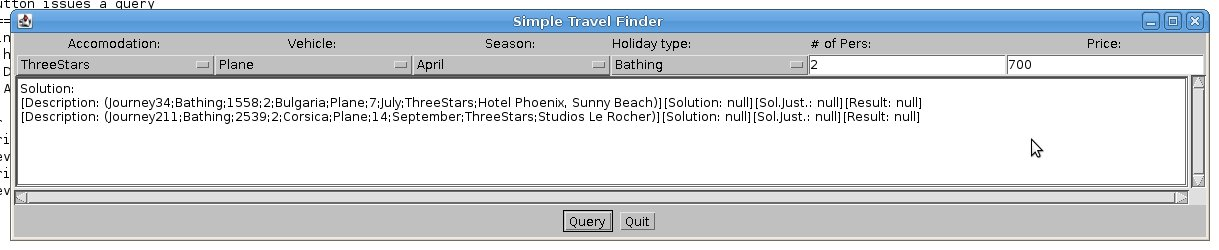
\includegraphics[scale=0.3]{exampleRun.jpg}
\caption{A GUI dummy for our Retrieval}
\label{fig:gui}
\end{figure}

\subsection{Problems}
Our implementation has some drawbacks in the creation of the Footprint set. The problem is, that it takes a lot of time. We perform a lot of comparisons inbetween the cases and don't have an optimal distance measure. For practical applications it might not even be a serious problem, that the creation of the Footprint set takes a lot of time. Usually we need to perform this important part of our retrieval approach only when the casebase is changed. Thus queries will be handled in an appropriate timeframe.


\section{Experimental Results}

\subsection{Random Distance}
To increase the speed of the Retrieval and check the creation of the Footprint set we first set random distance values for the comparison of two cases of our Travelcasebase. 

The most important part of the Footprint set creation is the selection of the Competencegroups. For a bunch of random distance cases it is very unprobable to fall within one and the same Competence group since two conditions must be hold:
\begin{itemize}
\item{group must be maximal in the sense that there are no other cases in the case-base that share coverage with any group member}
\item{each case in a competence group must share coverage with some other case in the group}
\end{itemize}
Trivially if we just assign random values it is very unlikely to happen, that a single case fulfills these condition. Therefore we have 1022 Competencegroups for 1024 cases in our casebase and the retrieval results are not very good.

\subsection{Global Similarity Measure}
With utilization of the given Global Similarity Measure the quality of the Footprint set increases.

\begin{figure}[h]
\begin{verbatim}
...
creating ReachabilitySet(c) ... Done.
RelatedSet: creation - Start.
Done.
Creating CompetenceGroups - Start
Creating CompetenceGroups - Ende (created 961)Number of CompetenceGroups: 961
Creating CompetenceGroup Footprints - Ende (total created + 961)
Number of CompetenceGroupsFootprints: 961
... creation of Footprintset completed!
FP set built.........
GUI will idle now...:
button is clicked...
gui Button issues a query
===========================================================================
 Running cycle with query:
Query has been issued with:
Query Description:
(null;Bathing;700;2;null;Plane;null;April;ThreeStars;null)

Number of CompetenceGroups: 961
Footprintsize: 994
Retrieved cases:
[Description: (Journey34;Bathing;1558;2;Bulgaria;Plane;7;July;ThreeStars;Hotel Phoenix, Sunny Beach)][Solution: null][Sol.Just.: null][Result: null]
[Description: (Journey211;Bathing;2539;2;Corsica;Plane;14;September;ThreeStars;Studios Le Rocher)][Solution: null][Sol.Just.: null][Result: null]
retrieval complete...
button is clicked...
gui Button issues a query
===========================================================================
 Running cycle with query:
Query has been issued with:
Query Description:
(null;Active;700;2;null;Coach;null;August;TwoStars;null)

Number of CompetenceGroups: 961
Footprintsize: 994
Retrieved cases:
[Description: (Journey841;Active;748;2;Slowakei;Car;7;January;TwoStars;Hotel Sverma, High Tatra)][Solution: null][Sol.Just.: null][Result: null]
retrieval complete...
\end{verbatim}
\caption{Console Output}
\label{fig:output}
\end{figure}


\subsection{Quality of Retrieval}
In contrast to other retrieval methods our Footprint approach will not necessarily return as much possible solutions to our query. After scanning the Footprint set the algorithm will only select possible candidates from the suited Competencegroup which might not be containing so many members. Especially in the Traveldataset and 1024 members, we get 961 Competencegroups with one member on average (refer to results in Figures \ref{fig:output} and \ref{fig:gui}).\\[1em]


\subsection{Speed of Retrieval}
If we do not consider the time for the creation of the Footprint set the Retrieval for a single query yields about the same time as the Retrieval in our Footprint-based implementation.

\section{Conclusion}
As a final conclusion we can state, 
TODO: Saurabh


%
% Literature / References
%
%\newpage
\nocite{FPBR}
\nocite{FPBR2}
\bibliographystyle{alpha}
\bibliography{mbr-bib}

%
% End of File
%
\end{document}
